\section{TRUST EVALUATION TESTING AND VERIFICATION}
\label{sec:geolocation}
%Description of the OBD system, how data can be retrieved from the car.
Another form of verification is the use of sensors on multiple devices~\cite{ju2012neteye}.  For example,
a smartphone may communicate directly with a smartwatch or on-board diagnostics (OBD)
sensor on an automobile.  These other devices have sensor with the same
functionality as some of the sensors on the smartphone.
% describe what data is collected, how it is stored, and how it might be used.
% we can include a graph of spped error vs time and the picture of the car route
We introduce a case where smartphones communicate with an in-vehicle OBD sensor
to get geolocation information, such as speed, engine RPM, fuel consumption, 
etc.

\subsection{Vehicle data collection}

Vehicular data collection consists of a process on a mobile 
device that directly communicates with in-vehicle sensors and collects sensor 
data~\cite{sensor}. Data can be encrypted and transferred to a
centralized server for permanent data storage. 
To deploy such a process on a mobile device, a device owner first installs an
app~\cite{sensor-app} on their devices\footnote{Currently, Android smartphones 
and tablets are supported.}. Since we are interested in
vehicular data, the target group of device owners are also vehicle 
owners. These owners simply insert their WiFi On-Board Diagnostics 
(OBD)~\cite{obd} sensor into their cars' OBD ports (located under the steering wheel),  
%\linda{I don't think they insert their sensor into the car. Do they insert it into something specific in the car (e.g., a usb port)? That would make sense. Anyway, I think you need to be more specific in stating what gets connected to what} 
and connect their 
smartphone or tablet to the sensor, which also runs as a WiFi access 
point. Note that OBD systems are in most cars and light trucks 
on the road today~\cite{obdconnector}. 
\eat{Therefore, our 
infrastructure does not require extra installation of specialized  
hardware or equipment~\cite{reininger2015first}. } % end comment
Trust evaluation could be used to determine if the phone should trust the car,
vice versa, as well as whether the user should trust the combined system.

The vehicular data is uploaded by the app
which runs in the background of the mobile device and communicates
with an in-vehicle OBD sensor. Device owners need not worry about having to
interact with the app or about being interrupted as they use their smartphones. 
Note that all code runs in a secure sandbox in our 
app~\cite{sensor-app}, which limits the amount of storage, network, 
memory, battery, and CPU resources used by any code~\cite{Cappos_CCS_10}. 
To protect end users' devices from malicious attackers, the sandboxed 
code is securely isolated from other programs on the same device.
Any bugs in the code will be contained in the sandbox, and will not 
affect the rest of the user device~\cite{Cappos_CCS_10}. 
%Once our prototype data collection application is installed and running on an Android smartphone with Sensibility, the end user need not worry about interacting with a user interface on the Android. Rather, once the user inserts their WiFi OBD sensor into the car and connects their Android smartphone to the sensor running as a wifi access point, our 
%

At the remote server, the vehicular sensor data collected from 
multiple end user devices is stored in a non-relational database. 
An example of 
collected data is shown in Figure~\ref{fig:json}, in JSON format.
The collected data set can be visualized on Google Maps to 
identify fuel efficient routes, routes with higher traffic activity, 
but it could also be used to detect reckless or illegal driving behaviors,
in which case trust metrics would be significant.

\eat{
\begin{figure}
\scriptsize 
\begin{Verbatim}
\{
  \textbf{"sensors"}: \{
    \textbf{"speed_car"}: \textcolor{red}{60},
    \textbf{"maf_car"}: \textcolor{red}{4},
    \textbf{"rpm_car"}: \textcolor{red}{114},
    \textbf{"gps_phone"}: \{
      \textbf{"error"}: \textcolor{red}{null},
      \textbf{"id"}: \textcolor{red}{0},
      \textbf{"result"}: \{
        \textbf{"network"}: \{
          \textbf{"time"}: \textcolor{red}{1407200660927},
          \textbf{"speed"}: \textcolor{red}{60},    
          \textbf{"altitude"}: \textcolor{red}{4.099999904632568},
          \textbf{"bearing"}: \textcolor{red}{82.6999694824219},
          \textbf{"provider"}: \textcolor{OliveGreen}{"gps"},
          \textbf{"longitude"}: \textcolor{red}{-73.986706},
          \textbf{"latitude"}:\textcolor{red}{40.694010},
          \textbf{"accuracy"}: \textcolor{red}{7},
        \}
      \}
    \},
    \textbf{"id"}: \textcolor{OliveGreen}{"310410696731709"},
    \textbf{"time"}: \textcolor{SkyBlue}{"ISODate"}(\textcolor{OliveGreen}{"2014-08-05T21:04:07.183-04:00"})
\}
\end{Verbatim}
\caption{JSON document of vehicular data.\label{fig:json}}
\end{figure}
}  % end comment


\eat{
\subsection{Data store}
Given the variety of sensors on a smartphone,
sensor measurements come in different forms. 
As shown in Figure~\ref{fig:json}, many types of sensor data have complex structure.
As a result, we decided to use a non-relational database, 
MongoDB~\cite{mongodb}, for storing sensor data. MongoDB has a Binary 
JSON (BSON) document-style structure identical to that shown previously 
in Figure~\ref{fig:json}, albeit converted into binary as its name suggests. 
This provides the scalability that is crucial to our system and that allows dynamic storage of 
new sensors, as needed. } % end comment

\subsection{Geolocation data analysis}

\begin{table}
\scriptsize
\centering
\begin{tabular}{|p{.06\columnwidth}|p{.18\columnwidth}|p{.22\columnwidth}|p{.28\columnwidth}|}
\cline{2-4}

%\multirow{3}{*}{Statistics}

\multicolumn{1}{c|}{}  & \textbf{GPS speed} & \textbf{Vehicle speed} & \textbf{Speed difference}  \\ \hline

% Mean & 5.559 & 1.568 & 0.003606 \\ \hline 

Med & 53.0~kph & 54.9~kph & 2.15~kph \\ \hline

STD & 12.79~kph & 13.61~kph & 4.57~kph  \\ \hline

\end{tabular}
\caption{\small Speed comparison: GPS speed comparing to OBD speed.}
\label{tab:speed-diff}
%\vspace*{-15pt}
\end{table}

\begin{figure}
\centering
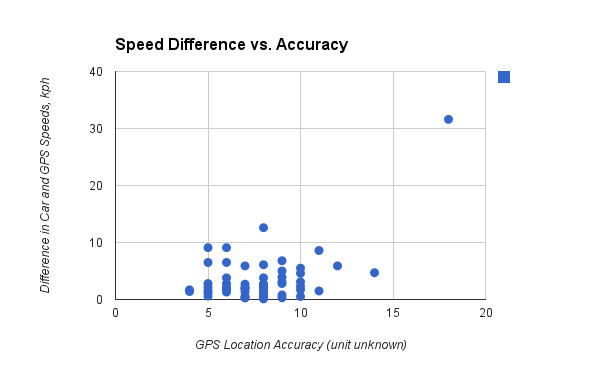
\includegraphics[width=3.5in]{speed.png}
\caption{Speed difference and accuracy.}
\label{fig:speed-diff}
\end{figure}

Using the aforementioned measurement, we collected speed data from both GPS 
on the smartphone inside a vehicle, and the speed via the OBD sensor. 
The data from these two sources can corroborate to verify normal or abnormal 
geolocation data. Table~\ref{tab:speed-diff} shows the median and standard deviation
of the speed measured by GPS and OBD sensor, over 58 data samples collected. 
The overall statistics do not show any anomaly in speed. However, when plotting 
individual data samples, we can see a data outlier in Figure~\ref{fig:speed-diff}. 
Excluding this point, the rest of the data samples roughly follow a Gaussian 
distribution. This outlier seems to be due to the initialization of the
GPS sensor.  Initially, the GPS parameters are underconstrained leading to a large 
geolocation error, which is rapidly reduced as more measurements are made.


\begin{figure}
\centering
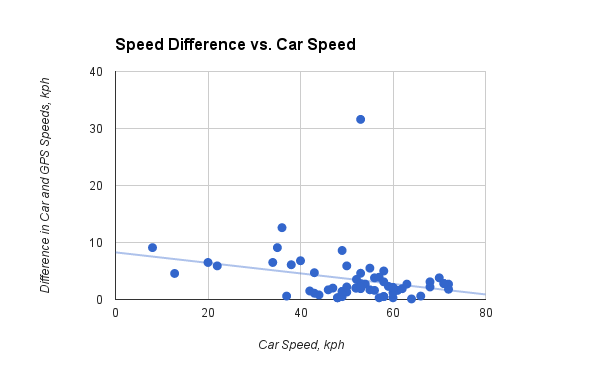
\includegraphics[width=3.5in]{car.png}
\caption{A typical session in Traceview, the execution log viewer.}
\label{fig:car}
\end{figure}

To further investigate on the speed data, we plot the differences between 
vehicle speed and GPS speed, and compare the differences against 
the varying vehicle speed. As shown in Figure~\ref{fig:car}, the speed 
differences are in a linear relation with the vehicle speed 
(other than the outlier), i.e., the 
higher the vehicle speed, the smaller difference between vehicle 
speed and GPS speed. 
The linear relationship in the figure is based on minimum mean 
square error (MMSE).

\begin{figure}
\centering
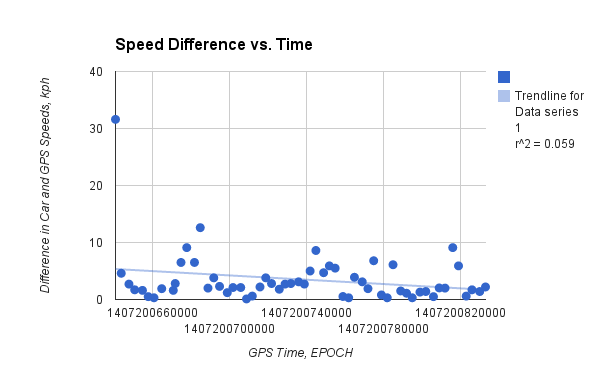
\includegraphics[width=3.5in]{time.png}
\caption{A typical session in Traceview, the execution log viewer.}
\label{fig:time}
\end{figure}

We also investigate the speed differences over time. 
In Figure~\ref{fig:time}, we can conclude that excluding the outlier, 
the differences between 
vehicle speed and GPS speed fluctuate around a constant value over 
time. 

\subsection{GPS Data}
\eat{
1) Overview of the Solution: Today's smartphone OS typ-
ically exposes resources based on a static policy. Such per-
missions are often much more than necessary. Several related
work has been proposed to refine or reduce permissions on
mobile platforms [18], [29], [17], [30] via modifying the
device platform. BlurSense allows untrusted parties to add
privacy filters from user space. Multiple security vendors
can efficiently and effectively collaborate to strengthen user
privacy.} %end comment

BlurSense provides a way to control the precision and accuracy of the GPS
sensor.  We show how blurring the GPS location affects the difference between
speed measured by a car speedometer and communicated via the OBD port to
a smartphone, similar to our experiment in section~\ref{sec:geolocation}.

\begin{figure}
\centering
%\includegraphics[width=3.5in]{}
\caption{Speed difference vs time with blurring of the GPS data.}
\label{fig:blur-GPS}
\end{figure}


\eat{
 BlurSense
provides a programmable privacy protection framework. Users
not only gain full transparency of what information is captured
on their devices, but also have full control over how much
information they would share with the rest of the world -
a secure personal data ecosystem. After installing BlurSense,
a user can install software from a third party (like a security vendor) that performs custom sensor filtering actions in
response to application requests. For example, an application
could be prevented from using motion sensors when running
in the background, or precise GPS data could be abstracted
to a neighborhood or zip code. 
BlurSense
provides effective controls for smartphones, much like Flash and JavaScript
filtering tools protect laptops and desktops (e.g., NoScript~\cite{noscript},
AdBlock~\cite{adblock}, FlashBlock~\cite{Flashblock}). 

2) What BlurSense Provides: Seattle provides a sensor
interposition mechanism and a sandboxing mechanism that
make it easy to implement privacy filters. A user can let a third
party have access to their sensor data from within a security
and performance isolated container [20]. By leveraging this
security, the user provides minimal trust in the third party,
but allows them an easy way to code their filters. This
functionality also automatically handles multiple privacy filters
from different parties through the sandbox policy composition
functionality~\cite{Cappos_CCS_10}.
Researchers who use BlurSense will build a mechanism
to trap the requests from generic  applications and pass them
into BlurSense (a proof-of-concept for Android has already
been built). They will build and manage an ``App Store'' for
BlurSense to allow users to locate privacy filters they wish
to apply. These may range from sharing sensor data with
researchers by reducing the precision of sensor values, salting
and hashing sensor values for anonymizing collected data,
or completely denying access to individual (or all) sensors.
For a particular sensor, a filter might perform an action such
as blurring the resolution of photos and video taken by the
camera, removing access point information from WiFi scans,
or omitting the motion sensor data completely. Security and
privacy groups can easily build and disseminate their own
privacy filters they recommend to users by adding them to
BlurSense app store. Therefore, BlurSense is able to handle
the three categories of threats in Section


\eat{To protect smartphone users'
privacy, Blursense provides a dynamic, fine-
grained, flexible access control mechanism, which incorporates
privacy filters in user space [19], [20]. } % end comment

We want to let users
choose defenses freely in a marketplace so that different
vendors can build them.
Specifically, it implements a framework of reference
monitors, to enforce mandatory access control to sensor data
in real time. A reference monitor is a method or function that
implements an access control policy for a set of resources and
is usually specified in terms of what capabilities are allowed.
The access control that we are concerned with in this paper is
for sensor data with respect to applications in user space. If
such an application needs to access any of the sensor data, the
second line of defensive (reference monitors) will come into
play, mediating every access to sensor data. 
%As a result, a user should be able to combine solutions from different vendors.
If a vendor's product is vulnerable to attack or the vendor is malicious,
the user can still be protected.
According to the semantics of the access requests and the
current context, when a remote procedure call is made to the
Android OS to request sensor data, it will be handled by a
reference monitor. Based on a sensitivity of the application,
the data returned may be filtered, dropped or passed through.
Note that the reference monitor cannot pass on data that is
blocked by the manifest file because it is layered on top of
whatever privacy and security mechanisms that are in place at
the OS level. If the request is for highly sensitive sensor data,
then the request might be simply rejected. Otherwise, if the
request is for medium-level sensitive sensor data, the request
might get through, but the returned data has reduced resolution.
If the request is for low-sensitive sensor data, then the return
results need to be processed, e.g., by filtering or obfuscation.
BlurSense can be used with Sensibility Testbed~\cite{cappos-sensibility}, 
which provides
a rich and extensible collection of sensor data from Android
devices 
}
